\begin{enumerate}
	\item From 
		\eqref{prop:lin-eq-unit-mat},
\begin{align}
\myvec{1&1&-1\\ 6&4&-5\\ -4&-2&3} \vec{n} = \myvec{1\\1\\1}
\end{align}
\begin{align*}
	\implies \myvec{1&1&-1&\vrule&1\\6&4&-5&\vrule&1\\-4&-2&3&\vrule&1}
	\\
\xleftrightarrow[R_3 \leftarrow R_3 + 4R_1]{R_2 \leftarrow R_2 - 6R_1}
\myvec{1&1&-1&\vrule&1\\0&-2&1&\vrule&-5\\0&2&-1&\vrule&5}\\ 
\xleftrightarrow[{R_1 \leftarrow 2R_1 + R_2}] {R_3 \leftarrow R_3 + R_2}
\myvec{2&0&-1&\vrule&-3\\0&2&-1&\vrule&5\\0&0&0&\vrule&0}
\end{align*}
Since we obtain a 0 row, 
the given points are collinear.
The direction vector of the line is
\begin{align}
\vec{m}=\vec{B}-\vec{C} \equiv \myvec{5\\3\\-4}
\end{align}
and the equation of a line is given by,
\begin{align}
	\vec{x}&=\vec{A}+  \kappa\vec{m}\\
&= \myvec{1\\1\\– 1} + \kappa \myvec{5\\3\\-4}
\end{align}
See 
     \figref{fig:chapters/12/11/3/6/1}.
\begin{figure}[H]
  \centering
   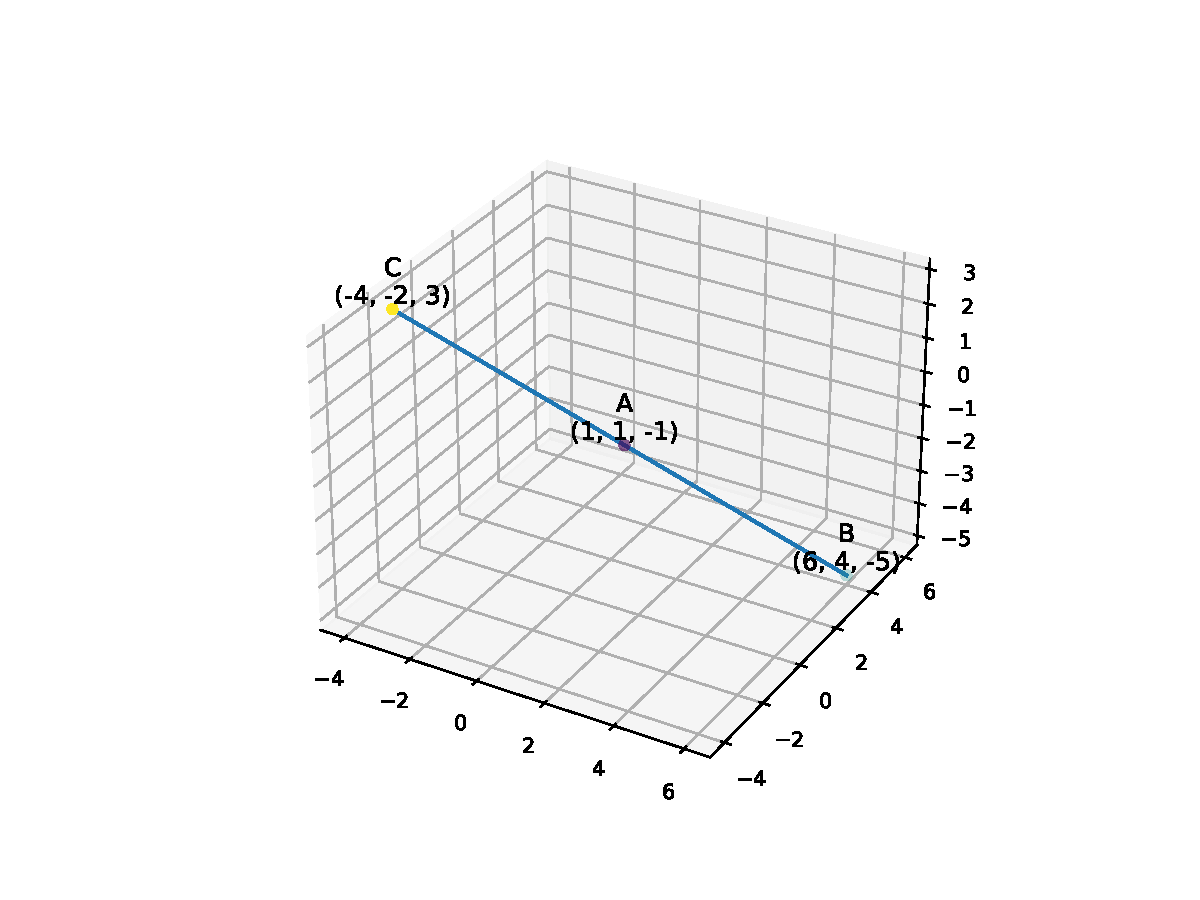
\includegraphics[width=0.75\columnwidth]{chapters/12/11/3/6/figs/fig.pdf}
    \caption{}
     \label{fig:chapters/12/11/3/6/1}
     \end{figure}
     \item  In this case, 
\begin{align}
\myvec{1&1&0 \\ 1&2&1 \\ -2&2&-1} \vec{n}=\vec{1}
\end{align}
\begin{align*}
\implies
\myvec{1&1&0&\vrule&1\\1&2&1&\vrule&1\\-2&2&-1&\vrule&1}
\\
\xleftrightarrow[R_3 \leftarrow R_3 + 2R_1]{R_2 \leftarrow R_2 - R_1}
\myvec{1&1&0&\vrule&1\\0&1&1&\vrule&0\\0&4&-1&\vrule&3}
\\
	\xleftrightarrow[R_3 \leftarrow R_3 - 4R_2]{R_1 \leftarrow R_1- R_2}
\myvec{1&0&-1&\vrule&1\\0&1&1&\vrule&0\\0&0&-5&\vrule&3}\\
	\xleftrightarrow[R_2 \leftarrow 5R_2 + R_3]{R_1 \leftarrow 5R_1- R_3}
\myvec{5&0&0&\vrule&2\\0&5&0&\vrule&3\\0&0&5&\vrule&-3}
\end{align*}
Hence, the equation of the plane is
\begin{align}
\myvec{2 & 3 & -3} \vec{x} = 5
\end{align}
\end{enumerate}
